\chapter{Semantic Analysis}
\label{chap:semantic_analysis}

With semantic analysis we begin the next step of our pipeline. We begin the
semantic analysis with an AST.

\section{Introduction}
    Semantic analysis allow us to check everything that :
    \begin{itemize}
        \item Can be check statically (without running the program) in
        reasonable time (no real symbolic execution (instead of real input, we
        use variable. The problem is when we encounter if branching because it
        multiply the amount of path (exponential) this phenomenon is called
        combinatorial explosion))
        \item That we didn't check in the parser (we should check as little as
        possible in the parser)
    \end{itemize}
    \subsection{Check after parsing}
        We can take the example of Java modifiers if we would like to check that
        in the parser we would need many rules, for each modifiers, the methods
        without them, etc. Thus, it would only be for non-abstract classes as
        the other (like interface) have other constraints. Besides, it does not
        prevent thing like "protected static" which is forbidden in Java.

        A first better way is to use Autumn parsing combinator, but still we
        should check that with the semantic analysis. An example of error for
        the following : public private void test()[] would be : 
        \begin{itemize}
            \item Parser : "unexpected token 'private'"
            \item Semantic: "two visibility modifiers for method"
        \end{itemize}
        No need to say that the second one is much better. Also, incorrect ASTs
        can be use in IDEs (syntax highlighting, etc.)
    \subsection{Main Concerns}
        \subsubsection{Type checking}
            \theoremstyle{definition}
            \begin{definition}[Type checking]
                Check type constraints : "int x = "String";" but also type
                inference : "var x = "string" + 42.
                If the language is dynamically typed it is done during runtime and libraries.
            \end{definition}

        \subsubsection{Name Binding}
            \theoremstyle{definition}
            \begin{definition}[Name binding]
                Check where name are defined. e.g : "int x = y + 3;" What is y?
                Inter-dependency : "var x = a.b.c" we need to know the type of
                c, that need the type of b, that need the type of a.
            \end{definition}
            These two first principle cannot be done separate.

            Note that Name binding also consist of lexical scoping (what is
            visible or not for a field/inside a method/block etc.). Dynamic
            scoping can also be done, however is it opposed with lexical
            scoping. Still it have this advantages! Emacs use this kind of
            scoping, this allow Emacs to edit Ruby and Python file and handle
            tabulation in both case.
        \subsubsection{Flow checks}
            Flow checks is a complex think, let's take a Java example : 
            \begin{lstlisting}[language=Java,label={lst:flow_check}]
                int test(int x) {
                    if (x == 3) return 3;
                }
                int test2(int x) {
                    while(true) return 1337;
                }
            \end{lstlisting}
            The first one is an invalid Java program (suppose to return an int
            but only return it if x==3) and flow checks spot that. The second
            one is valid because Java detects that the while loop will always be
            entered.
        \subsubsection{More...}
            Languages like Whiley / Dafny / Rust that statically does thinks.
\section{The Hindley-Milner Type System}
    \subsection{Introduction}
        Type system for polymorphic lambda calculus (System F). It is used in
        practice as it is the base of Haskell and ML type system. Also it can be
        extended in various ways.
    \subsection{Lambda calculus}
        \subsubsection{Lambda calculus}
            Toy language that is written this way : 
            $e::= x | (\lambda x.e) | (e e)$ variable/Abstraction/application

        \subsubsection{Simply-Typed Lambda calculus}
         $e::= x | (\lambda x:\tau.e) | (e e) | c$ where $\tau$ us the
        parameter type and c a constant. Note that, we need a set of base types
        e.g B = \{a, b\}. We do need constant c, because unlike classical lambda
        calculus we do not have the Church encoding (define number as function).

        \subsubsection{Polymorphic lambda calculus}
            The idea is to type the original lambda calculus without the type
            annotations \\ $e ::= x | (\lambda x.e) | (e e) | let x = e \text{ in } e$
    \subsection{Type system}
        \theoremstyle{definition}
        \begin{definition}[Type system]
            A formal system(formalism) that determines :
            \begin{itemize}
                \item if any expression in the language is well-typed
                \item type of any such expression
                \item $e::= x | (\lambda x:\tau .e) | (e e) | c$
                \item ill-typed: $((\lambda x:a . x) c1)$ where c1 has type b
            \end{itemize}
        \end{definition}

        We would like the type system to be :
        \begin{itemize}
            \item \textbf{Decidability} : can make a decision
            \item \textbf{Soundness} : everything we can prove is true
            \item \textbf{Completeness} : we can prove everything that is true
        \end{itemize}
        However the Gödel's incompleteness theorem says that "No sound system of
        axioms describing natural number arithmetic can be complete". Still, if
        we look in practice, Java does not have any of the previous properties... 

        \subsubsection{For $\lambda$}
            \begin{figure}[H]
                 \centering
                 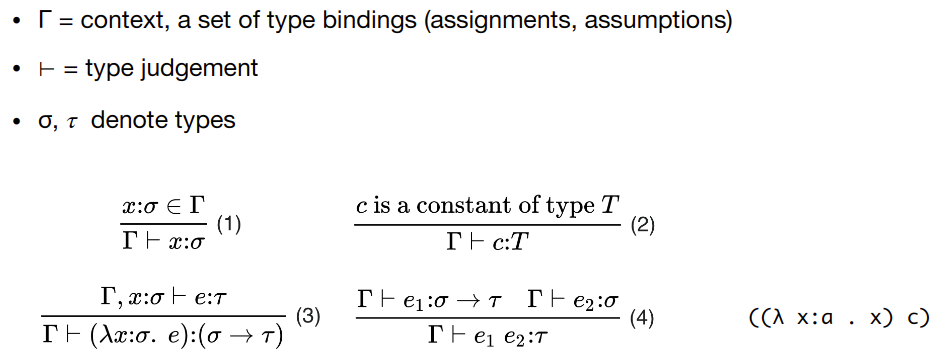
\includegraphics[scale=0.4]{type_system.png}
                 \caption{Type system for $\lambda$}
                 \label{fig:type_system}
            \end{figure}
    \subsection{Towards Hindley-Milner}
        The key idea is : function can have many types (polymorphism). Why is it
        important? Because we really need polymorphism in order to be able to
        write rule like $((\lambda id . ((foo (id 1)) (id 's'))) (\lambda x .
        x))$ without polymorphism, the identity function that we use should be
        declared as integer or char with polymorphism it can return both!

        \subsubsection{Generalization}
            \begin{figure}[H]
                \centering
                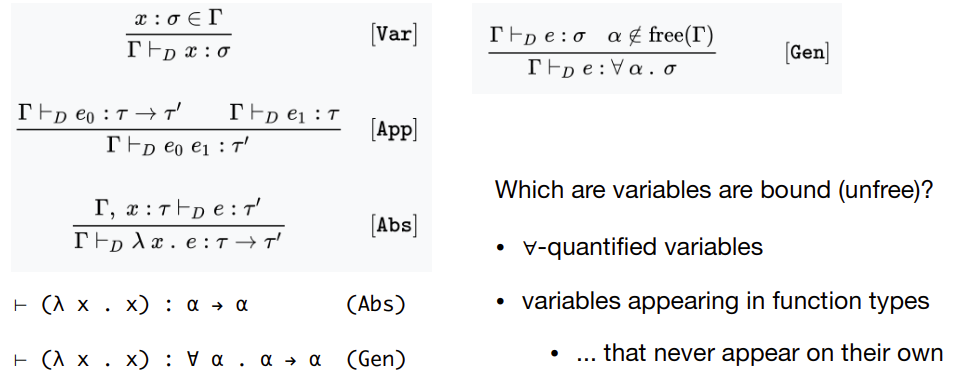
\includegraphics[scale=0.4]{Generalization.png}
                \caption{Generalization}
                \label{fig:Generalization}
            \end{figure}
            Still, it this step we cannot apply the function as we still have
            the polymorphic type and not a specialized type.
        \subsubsection{Intantiation}
            Allow us to specify a type from polymorphic type!
            \begin{figure}[H]
                \centering
                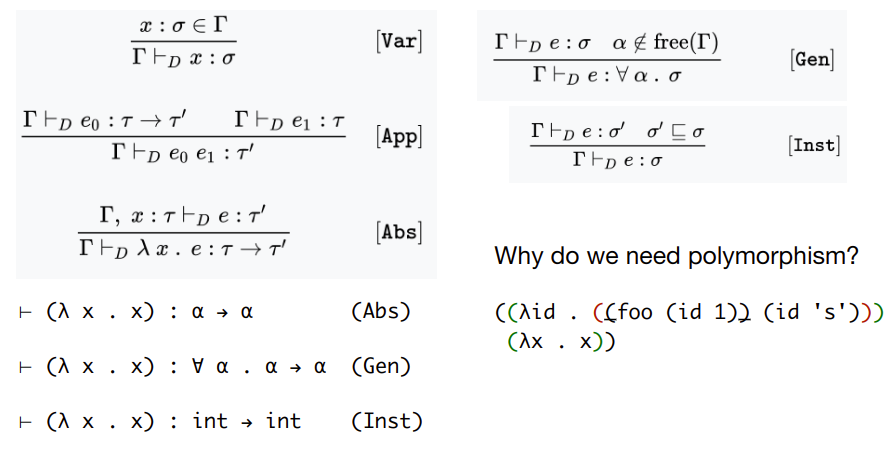
\includegraphics[scale=0.4]{Intantiation.png}
                \caption{Instantiation}
                \label{fig:instantiation}
            \end{figure}

        \subsubsection{Let polymorphism}
            The let rule allow us to go to a monomorphic type!
            \begin{figure}[H]
                 \centering
                 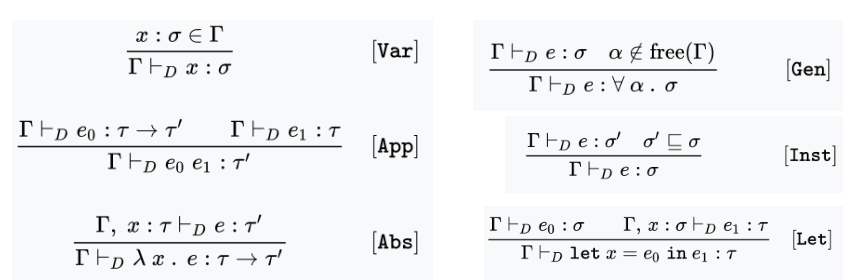
\includegraphics[scale=0.4]{let.png}
                 \caption{Let polymorphism}
                 \label{fig:let}
            \end{figure}
            We just need to rewrite it like : 
            $let id = (\lambda x . x) in ((foo (id 1)) (id 's'))$
    \subsection{Type system vs Typing algorithm}
        Thanks to inference rules we have the semantics of the type system.
        Rules allow us to prove statements about types, as the system is sound
        the created statements are true. However, the way to prove statements is
        not given (algorithm is needed for that). 
        
\section{Using Uranium}
\label{sec:using-uranium}

Uranium is a library written in Java. It is inspired by formal grammars,
attribute grammars and reactive programming. The goal of Uranium is the
specification of dependencies (using rules) e.g : "the type of a function call
depends on the type signature of the function being called, and on the type of
each of the arguments". Thus it is still explicit thanks to code computation and
verification of attributes.

    \subsection{Attribute grammars}
        The goal of attributes grammars is to calculate attributes on AST nodes.
        Many types:
        \begin{itemize}
            \item Synthesized attributes : computed from children node attributes
            \item Inherited attributes : computed from parent node attributes
            \item Combination of both
            \item Other have been proposed in practice 
        \end{itemize}

        It is called this way because it was originally designed within the
        grammar (which is a bad idea).
    
    \subsection{Uranium: Basics}
        Uranium computes attributes (AST Node, String) pair using rules:
        \begin{itemize}
            \item One or more dependency attributes
            \item One or more exported attributes
            \item Code that can read the dependency values, write exported values
            \item Automatically called when all dependency values are available
            \item All of this is done by the reactor
        \end{itemize}
        Check SemanticsAnalysis.java to have an example.
